\chapter{State of the art und Grundlagen}
Die Verkehrsstrategie des Senats sieht vor, dass das Radfahren bis zum Jahr 2025 20 Prozent des Gesamtverkehrs ausmachen soll. \cite{Mopo}
"Wir brauchen eine intelligente Konstruktion, die alle Verkehrsarten verbindet", sagte Stadtentwicklungssenator Michael Müller (SPD).\\
Sowohl statisch an Radwegen, als auch für den Einsatz in Kraftfahrzeugen gibt es bereits Projekte zu Ampelassistenten in Bordcomputern, Navigationssystemen, oder aber auch als App die rote Ampeln erkennen und die optimale Fahrtgeschwindigkeit für die Grüne Welle ermitteln.\\\\
\gls{V2X}- Kommunikation, GLOSA???\\
% ### Auto ###
\section{Bestehende Konzepte}
Unter dem Prinzip "'Grüne Welle'" wird die Abstimmung der Ampelschaltzustände, sodass ein Fahrzeug in einer bestimmten Geschwindigkeit mehrere Ampeln passieren kann ohne anzuhalten verstanden. Der folgende Abschnitt soll die existierenden Lösungen und Ansätze für die Empfehlung von Geschwindigkeiten an Lichtsignalanlagen darstellen.
\subsection{Grüne Welle auf Radwegen}
In Kopenhagen unterstützen grüne \gls{LED}s auf Radwegen die Radfahrer indem sie wenn diese mit einem Tempo von 20 km/h fahren, sie begleiten und so signalisieren, dass sie sich auf der Grünen Welle befinden. 
\begin{figure}[H]  
    \centering  
    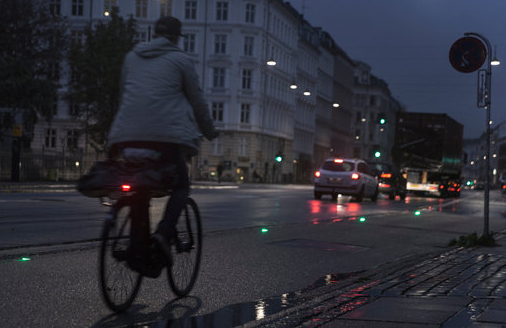
\includegraphics[scale=3]{copenhagen}
    \label{fig:copenhagen}
    \caption[Grüne Welle durch \gls{LED}s]{\gls{LED}s signalisieren die Grüne Welle bei 20 km/h  Quelle: \cite{NYT}}
\end{figure}
Zusätzlich erkennen Sensoren im Radweg Fahrradgruppen und veranlassen dann die Ampel zu einer längeren Grünphase. In einem anderen Stadtteil sind Leuchttafeln, die die verbleibende Zeit der Ampelphase anzeigen, am Fahrrand installiert\footnote{\cite{KopIng}}.\\
Mit Kopenhagen als Vorbild hat Berlin mit vier Ampeln in Schöneberg eine Grüne Welle für RadfahrerInnen umgesetzt und plant bereits die zweite\footnote{\cite{BZ}}. Auch hier möchte man die Benutzung des Rades attraktiver machen und den Fahrradverkehr beschleunigen.
\subsection{Projekt Wolfsburger Welle}
Die \gls{VW}-Forschung initiierte in den 80er Jahren mit dem Projekt "'Wolfsburger Welle"' die ersten Untersuchungen zur "'Grünen Welle"' Informationen im Fahrzeug; mit der Idee, beim Annähern an eine Ampel die optimale Geschwindigkeit im Fahrzeug zu geben.\footnote{\cite{Welle}} "Dazu sendet die Ampelanlage ihren aktuellen Phasenzustand und eine Prognose für den nächsten Zustandwechsel an alle Fahrzeuge, die sich annähern. Der Fahrzeugcomputer setzt dann die aktuelle Fahrzeuggeschwindigkeit mit dem Abstand zur Ampel und der aktuellen Ampelphase in Bezug. Daraus wird errechnet, ob das Fahrzeug im Moment mit der grünen Welle ’mitschwimmt’ oder ob die Geschwindigkeit außerhalb des optimalen Bereichs liegt" \cite{MenschMaschine}.
\subsection{Projekt Travolution}
Im Sommer 2008 wurde das Projekt TRAVOLUTION\footnote{\cite{Travolution}} (TRAffic \& eVOLUTION), von dem Amt für Verkehrsmanagement und Geoinformation der Stadt Ingolstadt, Audi AG\footnote{Automobilhersteller, dem Volkswagen-Konzern zugehörig}, GEVAS Software und dem Lehrstuhl für Verkehrstechnik an der \gls{TUM} abgeschlossen. Es besteht aus den Teilprojekten \textsc{verkehrsadaptive Netzsteuerung mit Genetischen Algorithmen} und \textsc{Der informierte Fahrer}. Im Netzsteuerungsprojekt wurden 46 Lichtsignalanlagen in Ingolstadt mit der Netzsteuerungssoftware BALANCE ausgestattet, wodurch sie intelligent auf den Verkehr reagieren und die Schaltung an den Verkehr anpassen. 
\begin{figure}[H]  
    \centering  
    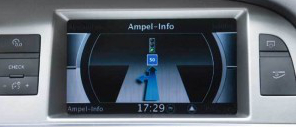
\includegraphics[scale=0.65]{audi-travolution}
    \label{fig:travolution}
    \caption[Projekt Travolution]{\gls{C2I}-Kommunikation: Der Bordcomputer zeigt die optimale Geschwindigkeit an, sodass die nächste Kreuzung ohne Halt überquert werden kann. Quelle: \cite{AudiTravolution}}
\end{figure}
Ziel des zweiten Teilprojektes ist es, die Autofahrer über die Ampelphasen zu informieren. Die \gls{C2I}-Kommunikation mittels WLAN umsetzend, senden mit Kommunikationsmodulen ausgestattete Ampeln die Grünphasen an den Bordcomputer der Autos, welcher widerum die Geschwindigkeit für ein reibungsloses Passieren errechnet.
\subsection{Projekt Testfeld Telematik}
Ende des Jahres 2013 wurde in Wien das Projekt Testfeld Telematik -- Feldversuch zur Stärkung österreichischen Know-Hows im Bereich umweltverträglicher Mobilität erfolgreich abgeschlossen. Per \gls{C2X}-Kommunikation\footnote{direkter Informationsaustausch zwischen Fahrzeugen jeglicher Art, Verkehrsleittechnik wie z.B. Lichtsignalanlagen und Verkehrsleitzentralen} bringt das Projekt unter Kooperative Dienste wie Ampelinformationen direkt ins Auto. Über Navigationssysteme, integrierte Systeme, Nachrüst-Plattformen oder mobile Endgeräte erreicht die FahrerInnen die Information der optimalen Geschwindigkeit sowie die Dauer der jeweiligen Ampelphase. Die Kommunikation zwischen den beteiligten Objekten verlief über ITS-GS, WAVE, CALM-IR und Mobilfunk.
\begin{figure}[H]
    \centering
    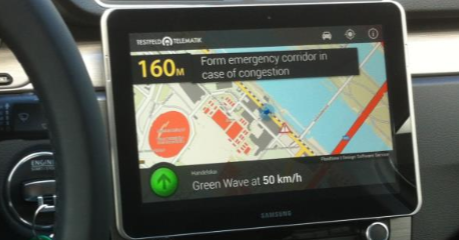
\includegraphics[scale=0.9]{telematik}
    \label{fig:telematik}
    \caption[Telematik Ampelinformation]{"'Grüne Welle bei 50 km/h'" Quelle: \cite{telematik}}
\end{figure}
Andere Autohersteller wie \gls{BMW}, Volvo und Volkswagen kooperieren als Forschungsprojekt "'Car 2 Car Communication Consortium'" mit Testfeld Telematik, ebenfalls mit dem Ziel die Sicherheit an Kreuzungen zu verbessern. Im Auto installierte Sensoren kommunizieren mit Kameras und Scanner in der Ampel. Allerdings funktioniert das System nur mit dem ambitionierten Ziel, wenn alle Autohersteller zusammenarbeiten und sich auf den gleichen Standard einigen.\footnote{\cite{Siemens}}
%%% KOLIBRI %%%
\subsection{Projekt Kolibri}
In Bayern wurde im April 2011 das Pilot-Projekt "'KOLIBRI'" (Kooperative Lichtsignaloptimierung -- Bayrisches Pilotprojekt) mit den Teststrecken der B13 bei München mit sieben und der St2145 in der Nähe von Regensburg mit acht ampelgeregelten Kreuzungen gestartet. Gemeinsam untersuchten TRANSFER GmbH\footnote{ein Beratungs- und Softwareunternehmen für Transport und Verkehr}, die \gls{BMW} Group, der Lehrstuhl für Ergonomie an der \gls{TUM} und die Oberste Baubehörde im Bayerischen Innenministerium die Funktionen und Auswirkungen eines Ampelassistenten außerhalb von Ortschaften\footnote{\cite{kolibri}, \cite{kolibriTUM}}. "'Per Mobilfunk übermittelt das Fahrzeug Rohdaten wie Zeit und genaue Position. Der Computer in der Zentrale kann daraus Informationen über die Verkehrslage, die Geschwindigkeit oder die Zahl der Ampelstopps und die Wartezeiten ermitteln, die dann als Korrekturgrößen wieder in die Steuerung der Lichtsignalanlage einfließen können.'"(\cite{kolibriTUM}) Zusätzlich wurden die Fahrer sowohl fahrzeugintegriert\footnote{On-Board-Computer} als auch via Smartphone über die Schaltung der nächsten Ampel informiert und erhielten Empfehlungen über die aktuelle Progressionsgeschwindigkeit. 
%%% AUTOS || TOYOTA %%%
\subsection{Autokonzerne}
Toyotas System erfordert eine spezielle Infrastruktur an Kreuzungen, die Installation von Infrarot-Sendern, die mit dem Toyota-Navigationssystem kommunizieren. An roter Ampel werden die Fahrer über die verbleibende Wartezeit informiert.\footnote{\cite{Toyota}}\\
%
%%% Apps %%% 
%
\section{Apps}
Ampelassistenten als App sind relativ unproblematisch. Smartphones sind bereits mit einem \gls{GPS}-Empfänger ausgestattet und haben fast durchgänging Internetzugang. Die hier vorgestellten mobilen Anwendungen existieren bereits oder befinden sich in der Testphase.
%%% ENLIGHTEN %%%
\subsection{EnLighten}
Die \gls{App} EnLighten erkennt rote Ampeln und visualisiert die Dauer dieser Phase. EnLighten nutzt \gls{GPS} zur Lokalisierung des Autos und verwendet die \gls{C2R}-Kommunikation zu Ampelphasenprognose.
\begin{figure}[H]
    \centering
    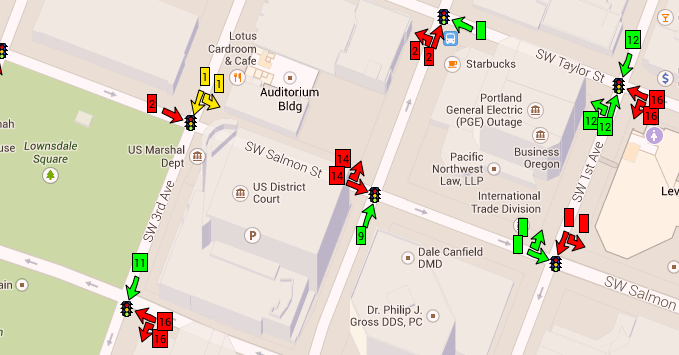
\includegraphics[scale=0.5]{EnLighten}
    \label{fig:Ampelsignalstatus}
    \caption[Echtzeit Ampelsignalstatus]{Schnappschuss der Echtzeit Ampelsignalstatusprognose in Portland. Quelle: \cite{EnLighten}}
\end{figure}
Hierbei verbindet sich die App über \gls{DSRC} mit den Lichtsignalanlagen und beachtet dabei Komponenten wie die Höchstgeschwindigkeit, Fahrtrichtung und Tageszeit. Die Installation der \gls{DSRC}-Hardware an den Komponenten ist sehr aufändig und teuer, weswegen EnLighten erst in einigen amerikanischen Städten funktionstüchtig ist.
%%% SIGNAL GURU %%%
\subsection{Signal Guru}
Signal Guru wurde von den Wissenschaftlern des \gls{MIT} und der Universität von Princeton entwickelt. Die App errechnet über die Smartphones vieler Nutzer - welche miteinander kommunizieren -  die Wahrscheinlichkeit, wann eine Ampel grün wird und wie das eigene Fahrverhalten entsprechend anzupassen ist. Wie in Abbildung \ref{fig:AppSignalGuru} ist zu sehen ist, muss die eingebaute Kamera durch die Windschutzscheibe die Ampel registrieren. Bei Testläufen im Straßenverkehr vielen die Ergebnise bei statisch geschalteten Ampeln deutlich besser aus als bei angepassten Ampelschaltungen \footnote{\cite{SignalGuru}} 
\begin{figure}[H]
    \centering
    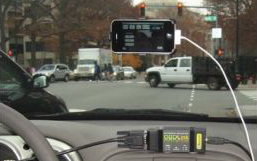
\includegraphics[scale=0.9]{SignalGuru}
    \caption[Signal Guru]{Signal Guru App muss in der Lage sein die Ampel zu 'sehen'.  Quelle: \cite{SignalGuruPaper}}
    \label{fig:AppSignalGuru}
\end{figure}
\textit{Ob das auch in Deutschland funktioniert ist schwer zu sagen, da die Ampeln hierzulande so gesetzt sind, dass das Smartphone in der Pole-Position die Ampel evtl. nicht erfassen kann. Dies gilt es in der Entwicklungsarbeit zu testen und gegebenenfalls auszuarbeiten.}
%%% AMPELMETER %%%
\subsection{Ampelmeter}
Ampelmeter ist eine Anwendung, die eine Geschwindigkeitsempfehlung angibt, bei der man die in Fahrtrichtung nächste Ampel bei grün erreichen. Der zweite Anwendungsfall ist die Restrot- bzw. Restgrünanzeige. Da der timingbezogene Teil der Datenbank zum Startzeitpunkt noch leer ist, bedarf es der Mitarbeit der NutzerInnen.
%%% ERGIBNIS %%%
\section{Analyseergebnis}
Diese Beispiele zeigen deutlich, dass die Nachfrage nach Ampelassistenten -- mobil oder statisch -- steigt und auf dem Markt Anklang findet. Der Verkehr ist flüssiger, die Teilnehmer entspannter, die Luft sauberer. AutofahrerInnen sind schon lange nicht mehr allein auf der Straße und so gilt es, dieses erfolgreiche Konzept für alle VerkehrteilnehmerInnen zu erweitern.
%
%
%%% Technische Grundlagen %%%
%
%
\section{Technische Grundlagen}
\subsection{Arduino / Android-App}
\subsubsection{Mobile Sensing}
\textit{Der Beschleunigungssensor ist ein Hardwaresensor, der dazu benutzt wird, Position, Bewegung, Neigung, Erschütterung, Vibration und natürlich Beschleunigung des Gerätes zu messen.Es gibt bis zu 3-Achsen Beschleunigungssensoren, die meistens zum Erkennen der Ausrichtung des Smartphones genutzt werden und somit das Display beim Anschauen von Bildern, Webbrowsern oder Musikplayern in die passende Richtung vom Portrait-Modus (senkrecht) zum Landscape-Modus (waagrecht) zu drehen. In Kombination mit \gls{GPS} kann das Smartphone dank ihm sogar erkennen, welche Art Transportmittel (Fahrrad, Bus, U-Bahn) der Nutzer gerade benutzt und bestimmte Muster wie z.B. Rennen, Gehen oder Stehen unterscheiden.\\
\gps{GPS} erlaubt dem Smartphone sich selber zu lokalisieren und den exakten Standpunkt auf der Erde zu bestimmen. Es hilft locationbased\footnote{ortsgebunden} Apps wie z.B Navigation, lokale Suche nach Shops, Restaurants etc. oder soziale Netzwerke wie Facebook oder Foursquare nötige Informationen zu ermitteln. Der Kompass erweitert die Möglichkeiten der Lokalisationsermittlung eines Smartphones. Er bestimmt den Winkel des Geräts relativ zum Nordpol der Erde. Der Kompass besitzt einen Magnet, der mit dem magnetischen Feld der Erde interagiert und sich entsprechend zu einem der Pole ausrichtet. Zusammen mit dem Gyroskop Sensor verbessern \gls{GPS} und Kompass die Präzision von locationbased Applikationen.Der Gyroskop Sensor bestimmt die Rotations- und Drehgeschwindigkeit des Smartphones auf seinen drei Achsen gegenüber dem Weltkoordinatensystem.}
\subsection{Backend mit nodejs / socket.io und MongoDB}
\subsection{Open-Street-Map}
